\documentclass[10pt,a4paper]{article}
\usepackage[a4paper,margin=2.1cm]{geometry}
\usepackage{amsmath}
\usepackage{fontspec}
\usepackage{polyglossia}
\setmainlanguage{russian}
\setotherlanguage{english}
\setmainfont{Liberation Serif}[Ligatures=TeX]
\newfontfamily\cyrillicfont{Liberation Serif}[Ligatures=TeX]
\newfontfamily\cyrillicfontsf{Liberation Sans}[Ligatures=TeX]
\newfontfamily\cyrillicfonttt{DejaVu Sans Mono}[Scale=0.82]
\setsansfont{Liberation Sans}
\setmonofont{DejaVu Sans Mono}[Scale=0.82]
\usepackage[italic,nopunctuation,nominus]{mathastext}
\DeclareSymbolFont{txtdig}{TU}{\rmdefault}{m}{n}
\DeclareMathSymbol{0}{\mathalpha}{txtdig}{"30}
\DeclareMathSymbol{1}{\mathalpha}{txtdig}{"31}
\DeclareMathSymbol{2}{\mathalpha}{txtdig}{"32}
\DeclareMathSymbol{3}{\mathalpha}{txtdig}{"33}
\DeclareMathSymbol{4}{\mathalpha}{txtdig}{"34}
\DeclareMathSymbol{5}{\mathalpha}{txtdig}{"35}
\DeclareMathSymbol{6}{\mathalpha}{txtdig}{"36}
\DeclareMathSymbol{7}{\mathalpha}{txtdig}{"37}
\DeclareMathSymbol{8}{\mathalpha}{txtdig}{"38}
\DeclareMathSymbol{9}{\mathalpha}{txtdig}{"39}
\usepackage{booktabs,graphicx,enumitem,xcolor,float}
\usepackage[font=small,labelfont=bf,labelsep=period]{caption}
\usepackage[colorlinks=true,urlcolor=black,linkcolor=black]{hyperref}
\sloppy\emergencystretch=3em
\setlength{\parindent}{0pt}\setlength{\parskip}{4pt plus 1pt}
\setlist{nosep,leftmargin=1.4em,itemsep=2pt}
\newcommand{\gr}{^{\circ}}
\newcommand{\ci}[2]{$[#1;\,#2]$}
\newcommand{\dsq}{\text{град}^2}
\renewcommand{\tablename}{Таблица}
\renewcommand{\figurename}{Рис.}

\AtBeginDocument{\mathcode`\,="013B \mathcode`0=\numexpr"7000+\symtxtdig*"100+"30\relax \mathcode`1=\numexpr"7000+\symtxtdig*"100+"31\relax \mathcode`2=\numexpr"7000+\symtxtdig*"100+"32\relax \mathcode`3=\numexpr"7000+\symtxtdig*"100+"33\relax \mathcode`4=\numexpr"7000+\symtxtdig*"100+"34\relax \mathcode`5=\numexpr"7000+\symtxtdig*"100+"35\relax \mathcode`6=\numexpr"7000+\symtxtdig*"100+"36\relax \mathcode`7=\numexpr"7000+\symtxtdig*"100+"37\relax \mathcode`8=\numexpr"7000+\symtxtdig*"100+"38\relax \mathcode`9=\numexpr"7000+\symtxtdig*"100+"39\relax }
\begin{document}

\begin{center}
{\Large\bfseries Дифференциальная модель стягивания к диагоналям:\\[2pt]
формулировка и проверка на данных Stein, Barbosa и соавт. (2020)}\\[6pt]
{\small Рабочая сводка результатов, 5 октября 2026 г. Продолжение сводки о проверке данных.}
\end{center}

\textbf{Коротко.} Закон <<стягивание пропорционально неопределённости>> можно получить двумя способами: как
блуждание следа памяти в потенциале, где снос пропорционален силе шума (дифференциальная модель, Д), или как сдвиг
неточного воспоминания к середине квадранта в момент ответа (модель О). Модели различаются тем, как случайный разброс
распределён по окружности, и эта величина в их настройку не входит. Модель О отвергнута во всех восьми сравнениях:
она завышает разброс у осей примерно вдвое. Модель Д даёт верный размер эффекта, но ни один из двух её вариантов не
прошёл проверку полностью: данные лежат между ними. На этих данных работа с моделью остановлена.

\section*{1. Откуда модель}

На независимых пробах проверено соотношение между силой стягивания $\lambda$ (доля пути от точки до ближайшей
диагонали, которую проходит ответ) и случайной дисперсией $V$:
\begin{equation}
\lambda(t)\bigl(1-\lambda(t)\bigr)=V(t)/V_p .
\label{eq:law}
\end{equation}
Снос с постоянной скоростью данным противоречит. Отношения в табл.~1 постоянны при всех трёх паузах, причём для обеих
форм записи, алгебраической и дифференциальной: при наблюдаемых $\lambda\le 0{,}13$ они различаются на несколько
процентов, что меньше погрешности.

\begin{table}[H]\centering\small
\caption{Проверка постоянства (арифметика по средним из отчётов; все люди).}
\begin{tabular}{llcccc}\toprule
Сессии & Пауза & $\lambda$ & $V$, $\dsq$ & $\lambda(1-\lambda)/V$ & $\lambda(2-\lambda)/V$\\\midrule
исходные & 0 с & 0,039 & 11,8 & 0,0032 & 0,0066\\
 & 1 с & 0,093 & 28,3 & 0,0030 & 0,0063\\
 & 3 с & 0,132 & 37,0 & 0,0031 & 0,0067\\\addlinespace
\texttt{post} & 0 с & 0,031 & 8,9 & 0,0034 & 0,0068\\
 & 1 с & 0,090 & 25,6 & 0,0032 & 0,0067\\
 & 3 с & 0,125 & 33,2 & 0,0033 & 0,0071\\\bottomrule
\end{tabular}
\end{table}

\section*{2. Две модели}

\textbf{Модель Д, дифференциальная.} Положение следа $x$ на окружности подчиняется уравнению
\begin{equation}
dx=-\frac{D(t)}{V_*}\,g(x)\,dt+\sqrt{2D(t)}\,dW ,
\label{eq:sde}
\end{equation}
где $g(x)$ --- форма стягивания (ноль на диагоналях и на осях), $D(t)$ --- сила шума. Снос не имеет собственной
скорости: он пропорционален шуму, и шум только задаёт темп приближения к равновесному распределению. Если ввести
<<диффузионное время>> $\tau(t)=\int_0^t D(s)\,ds$ и взять одну яму с $g(x)=x$, уравнение решается явно:
\begin{equation}
1-\lambda=e^{-\tau/V_*},\qquad V=V_*\bigl(1-e^{-2\tau/V_*}\bigr)=V_*\,\lambda\,(2-\lambda).
\label{eq:ou}
\end{equation}
При малых $\lambda$ это совпадает с~(\ref{eq:law}) при $V_p=2V_*$. По средним из табл.~1 получается
$V_*\approx150$--$155~\dsq$ (ширина ямы около $12\gr$) и $\tau\approx 6$, $16$ и $21~\dsq$ при трёх паузах: в первую
секунду $D\approx 9{,}5~\dsq$/с, далее около $2{,}8$.

\textbf{Модель О, подправка при ответе.} След только блуждает и к концу паузы имеет дисперсию $V_{\text{пам}}$; при
ответе он сдвигается: ответ $=m-\lambda\,g(m)$, где $\lambda=V_{\text{пам}}/(V_{\text{пам}}+V_p)$.

\textbf{Чем они различаются.} Пусть $s(x)=g'(x)$ --- местный наклон формы: положительный у диагоналей (поток
сходится), отрицательный у осей (расходится). В первом порядке по $\lambda$ местная дисперсия равна
\begin{equation}
V_{\text{Д}}(x)\approx 2\tau\,\bigl(1-\lambda\,s(x)\bigr),\qquad
V_{\text{О}}(x)\approx 2\tau\,\bigl(1-2\lambda\,s(x)\bigr).
\label{eq:two}
\end{equation}
Постепенное стягивание сжимает накопленный шум вдвое слабее, чем разовый сдвиг той же величины в конце: шум, пришедший
поздно, не успевает сжаться. Этот множитель два не зависит от деталей, поэтому профиль разброса по окружности
различает модели.

\section*{3. Как проверяли}

\textbf{Настройка.} У каждого человека по его данным берутся $\lambda(t)$ и общая дисперсия $V(t)$ при трёх паузах.
Параметр ямы ($V_*$ или $V_p$, один на человека) подбирается так, чтобы суммарное стягивание в модели равнялось
измеренному; количество шума при каждой паузе --- так, чтобы совпала общая дисперсия. Подбор идёт прогонами самой
модели: модельные пробы создаются в тех же местах окружности, что и настоящие (по 20 на каждую), и проходят тот же
расчёт. Распределение дисперсии по окружности в настройке не участвует.

\textbf{Проверяемые величины.} Дисперсия остатка в трёх полосах расстояния до диагонали: $0$--$15\gr$ (у диагонали),
$15$--$30\gr$ (середина), $30$--$45\gr$ (у оси), и два отношения к полосе у диагонали.

\textbf{Правило} записывалось до расчёта: модель совместима, если $99\,\%$ интервал разности <<данные минус модель>>
содержит ноль во всех сравнениях при паузах 1 и 3~с (бутстрэп по людям). Основная проверка --- исходные сессии
(52 человека), сессии \texttt{post} (22 человека) --- справочно.

\textbf{Два круга.} В первом круге (\texttt{wm\_stein7.py}) форма была пилой, $g(x)=\delta(x)$, со скачком на осях;
проверялось только отношение <<у оси / у диагонали>>. Модель Д не прошла при паузе 3~с. Во втором круге
(\texttt{wm\_stein8.py}) форма задана гармониками 4, 8 и 12 и подстроена так, чтобы средняя карта смещений в модели
совпала с измеренной; проверялись оба отношения. Второй круг --- пересмотр после непройденной проверки, на уже
виденном профиле, и это записано в шапке скрипта.

\textbf{Проверка метода.} В обоих скриптах расчёт прогонялся на искусственных людях, порождённых одной из моделей.
После исправления ошибок настройки, найденных этим способом, метод называл породившую модель во всех четырёх мирах.

\section*{4. Результаты}

\begin{figure}[H]\centering
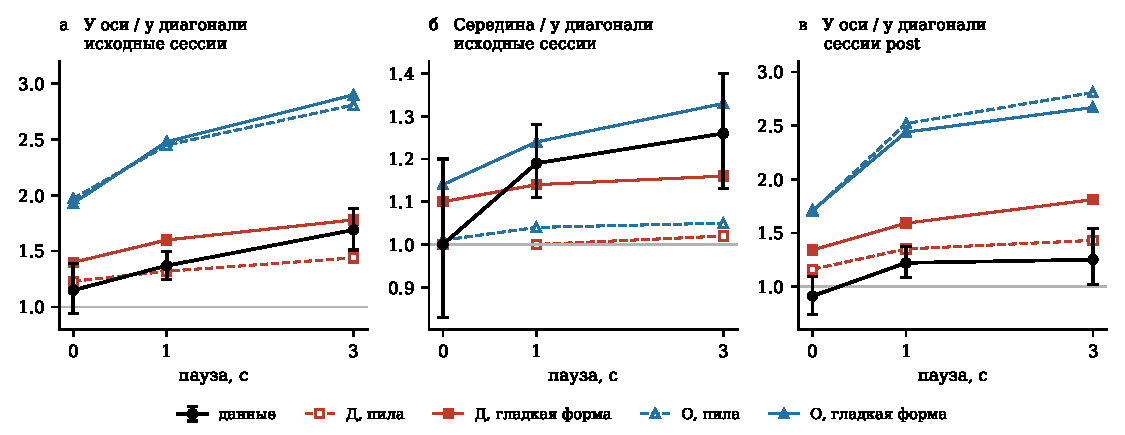
\includegraphics[width=\textwidth]{fig2.pdf}
\caption{Отношения дисперсий: данные (с $95\,\%$ интервалом) и четыре варианта моделей. Пауза 0~с справочная.}
\end{figure}

\begin{table}[H]\centering\small
\caption{Отношение <<у оси / у диагонали>>. Звёздочка: $99\,\%$ интервал разности с данными не содержит ноль.}
\begin{tabular}{llccccc}\toprule
Сессии & Пауза & Данные & Д, пила & Д, гладкая & О, пила & О, гладкая\\\midrule
исходные & 1 с & 1,37 \ci{1,25}{1,50} & 1,32 & 1,60$^*$ & 2,45$^*$ & 2,48$^*$\\
 & 3 с & 1,69 \ci{1,51}{1,88} & 1,44$^*$ & 1,78 & 2,81$^*$ & 2,90$^*$\\\addlinespace
\texttt{post} & 1 с & 1,22 \ci{1,08}{1,37} & 1,35 & 1,59$^*$ & 2,52$^*$ & 2,44$^*$\\
 & 3 с & 1,25 \ci{1,02}{1,54} & 1,43 & 1,81$^*$ & 2,81$^*$ & 2,67$^*$\\\bottomrule
\end{tabular}
\end{table}

\begin{table}[H]\centering\small
\caption{Отношение <<середина / у диагонали>>. Для гладкой формы все разности с данными совместимы с нулём; для пилы
это отношение в правило не входило.}
\begin{tabular}{llccccc}\toprule
Сессии & Пауза & Данные & Д, пила & Д, гладкая & О, пила & О, гладкая\\\midrule
исходные & 1 с & 1,19 \ci{1,11}{1,28} & 1,00 & 1,14 & 1,04 & 1,24\\
 & 3 с & 1,26 \ci{1,13}{1,40} & 1,02 & 1,16 & 1,05 & 1,33\\\addlinespace
\texttt{post} & 1 с & 1,12 \ci{1,00}{1,25} & 1,00 & 1,06 & 1,02 & 1,08\\
 & 3 с & 0,99 \ci{0,83}{1,17} & 0,99 & 1,09 & 1,03 & 1,11\\\bottomrule
\end{tabular}
\end{table}

\begin{table}[H]\centering\small
\caption{Дисперсия остатка по полосам в исходных сессиях, $\dsq$ (у диагонали / середина / у оси).}
\begin{tabular}{lccccc}\toprule
Пауза & Данные & Д, пила & Д, гладкая & О, пила & О, гладкая\\\midrule
1 с & 25,7 / 30,5 / 35,2 & 27,7 / 27,5 / 36,5 & 24,5 / 28,0 / 39,4 & 20,4 / 21,2 / 50,0 & 19,4 / 24,0 / 48,1\\
3 с & 29,2 / 36,6 / 49,3 & 33,6 / 34,3 / 48,5 & 29,7 / 34,5 / 52,9 & 23,6 / 24,9 / 66,3 & 22,1 / 29,5 / 64,1\\\bottomrule
\end{tabular}
\end{table}

\textbf{Вывод по правилу в обоих кругах на исходных сессиях: обе модели профиль не описывают.}

\textbf{Модель О отвергнута.} У осей она завышает отношение на $1{,}1$--$1{,}6$ во всех восьми сравнениях (две формы,
две паузы, два набора данных). Неверны и абсолютные уровни: при 3~с у осей $64$--$66~\dsq$ против $49$ наблюдаемых, у
диагоналей $22$--$24$ против $29$. Это согласуется с~(\ref{eq:two}): разовый сдвиг сжимает и растягивает разброс
вдвое сильнее, чем наблюдается.

\textbf{Модель Д: размер эффекта верен, форма профиля --- нет.}
\begin{itemize}
\item С пилой уровень у осей верен ($48{,}5$ против $49{,}3~\dsq$ при 3~с), но профиль ровный до самой оси: середина
не отличается от диагонали, а в данных она выше на $19$--$26\,\%$. Отношение у оси занижено при 3~с
(разность $0{,}25$ \ci{0{,}04}{0{,}50}). На сессиях \texttt{post} этот вариант совместим с данными при обеих паузах.
\item С гладкой формой середина описана (разности $0{,}05$ и $0{,}10$, интервалы содержат ноль), абсолютные дисперсии
при 3~с близки к наблюдаемым, но разброс у осей завышен: при 1~с разность $-0{,}23$ \ci{-0{,}38}{-0{,}08}; на сессиях
\texttt{post} --- $-0{,}37$ и $-0{,}56$. Знак разности одинаков во всех шести сравнениях, включая паузу 0~с.
\item Данные лежат между двумя вариантами: пила слишком плоская в середине, гладкая форма слишком крутая у осей.
\end{itemize}

\textbf{Измеренная форма.} В средней карте гармоника с 8 периодами составляет $0{,}24$ от гармоники с 4 периодами по
размаху, гармоника с 12 периодами --- $0{,}07$ (у пилы $0{,}50$ и $0{,}33$). Наибольшее стягивание приходится на
$30\gr$ от диагонали; наклон у диагонали около $2$, у оси около $-5$ в единицах наклона пилы.

\textbf{Параметры.} Медиана глубины ямы по людям: $V_*=124~\dsq$ с пилой и $139~\dsq$ с гладкой формой;
$V_p=169$ и $214~\dsq$.

\section*{5. Что ещё не сходится}

\begin{itemize}
\item \textbf{Пауза 0~с.} Когда памяти ещё нет, наблюдаемый профиль плоский (отношение $1{,}15$ и $0{,}91$), а модель Д
с гладкой формой даёт $1{,}40$ и $1{,}34$. Модель считает весь разброс блужданием в потенциале; часть его, вероятно,
обычный шум ответа, не зависящий от места. При этом само стягивание при 0~с есть и подчиняется~(\ref{eq:law}).
\item \textbf{Стягивание при 3~с} в обеих моделях получается меньше измеренного: $0{,}119$--$0{,}120$ (Д) и
$0{,}108$--$0{,}112$ (О) против $0{,}132$. Между 1 и 3~с стягивание растёт несколько быстрее дисперсии.
\item \textbf{Хвосты.} Распределения ошибок в данных островершиннее, чем в обеих моделях: в моделях нет ни промахов,
ни изменчивости точности от пробы к пробе.
\item \textbf{Поздний дрейф к оси $0$--$180\gr$} в модель не входит: он не идёт за шумом и требует отдельного члена.
\end{itemize}

\section*{6. Следствия модели, которые не проверялись}

\begin{itemize}
\item \textbf{Длинные паузы.} В модели Д дисперсия насыщается на уровне $V_*$ (около $125$--$155~\dsq$). В модели О
наблюдаемая дисперсия не превышает $V_p/4$ (около $40$--$80~\dsq$) и затем убывает. При паузах 10--20~с это разные
предсказания.
\item \textbf{Различия между людьми} в модели --- это разная глубина ямы, а не разный шум. Это согласуется с тем, что
связи между силой стягивания и случайной дисперсией у разных людей не найдено.
\item \textbf{Ход шума.} Диффузионное время в первую секунду идёт в три-четыре раза быстрее, чем потом. По трём
паузам форму $D(t)$ определить нельзя.
\end{itemize}

\section*{7. Ограничения}

\begin{itemize}
\item Второй круг проверки сделан после неудачи первого и на уже виденных данных; его положительные части весят
меньше, чем предсказание с первого раза.
\item Модель О проверена в двух вариантах (со скачком на осях и гладком). Другие способы подправки при ответе этим не
исключены.
\item Форма стягивания одна на всех людей; настройка каждого человека опирается на его собственные, зашумлённые
оценки $\lambda$.
\item Сессии \texttt{post} --- те же люди, что в исходных; больных шизофренией среди них нет.
\end{itemize}

\section*{Материалы}

{\small Данные: Stein H., Barbosa J. и соавт. \emph{Nature Communications} 2020; 11: 4250;
\texttt{github.com/comptelab/serialNMDA}. Расчёты: \texttt{wm\_stein7.py} (пила) и \texttt{wm\_stein8.py} (гладкая
форма); оба содержат проверку метода на искусственных данных. Закон~(\ref{eq:law}) и его проверка описаны в первой
сводке (\texttt{stein2020\_check.pdf}).}

\end{document}
